\section{Introduction}
\label{sec:introduction}

The Heavy Photon Search (HPS) prompt-resonance program is formulated in the minimal
visible dark-photon model, in which a new broken $U(1)_D$ gauge boson mixes
kinetically with the Standard-Model photon \cite{Holdom1986,EssigEtAl2011}. After
diagonalizing the gauge fields, the interaction terms relevant for the prompt
$A^\prime \rightarrow e^+e^-$ search can be written schematically as
\begin{equation}
\mathcal{L}
\supset
-\frac{1}{4}F_{\mu\nu}^{\prime}F^{\prime\mu\nu}
-\frac{\eps}{2}F_{\mu\nu}^{\prime}F^{\mu\nu}
\,+\,\frac{1}{2}m_{A^\prime}^{2}A_\mu^\prime A^{\prime\mu}
\,+\,\eps e J_{\mathrm{EM}}^\mu A_\mu^\prime .
\label{eq:dark-photon-lagrangian}
\end{equation}
Here $\eps$ is the kinetic-mixing parameter, $m_{A^\prime}$ is the dark-photon mass,
and $J_{\mathrm{EM}}^\mu$ is the ordinary electromagnetic current. In the low-mass
region considered here, the minimal visible model predicts a narrow prompt dielectron
resonance. Its natural width is negligible compared with the HPS detector resolution,
so the observed line shape is set by the experimental mass resolution
\cite{HPS2015DarkPhoton,HPS2016PromptLong}. This narrow-width regime makes a resonance
search well suited to the \SIrange{10}{300}{MeV} mass window: fixed-target
electroproduction can reveal a visibly decaying vector as a localized excess above the
smooth trident spectrum, in a coupling range that includes established dark-sector and
lepton-anomaly benchmarks.

In the fixed-target approximation relevant for HPS, prompt dark-photon production is
normalized to the radiative trident rate,
\begin{equation}
\sigma(e Z \rightarrow e Z A^\prime)
\simeq
\frac{3\pi \eps^2}{2\alpha_{\mathrm{EM}}}\,
m_{A^\prime}\,
\left.\frac{d\sigma_{\gamma^\ast}}{dm}\right|_{m=m_{A^\prime}},
\label{eq:ap-production}
\end{equation}
the analysis extracts a narrow signal yield from the smooth prompt $e^+e^-$ spectrum
and then converts that yield into a limit or best fit for $\eps^2$
\cite{EssigEtAl2011,HPS2015DarkPhoton,HPS2016PromptLong}. The physics interpretation
rests on the minimal prompt $A^\prime$ model and the radiative-trident normalization;
Gaussian-process regression (GPR) provides the statistical description of the smooth
background.

\subsection{Published HPS prompt-resonance benchmarks}

The published HPS prompt searches provide the immediate experimental context for the
current GPR analysis. The 2015 engineering-run publication analyzed
\SI{1170}{nb^{-1}} at \SI{1.056}{GeV} over \SIrange{19}{81}{MeV} and reported a lowest
local $p$-value of $1.7\times10^{-3}$ at \SI{37.7}{MeV}; after the look-elsewhere
correction the global $p$-value was 17\%
\cite{HPS2015DarkPhoton}. The 2016 prompt search analyzed the full engineering-run
sample, \SI{10608}{nb^{-1}} at \SI{2.3}{GeV}, over \SIrange{39}{179}{MeV}. Its lowest
local $p$-value was $6.38\times10^{-3}$ at \SI{94}{MeV}, with a global significance of
about $1\,\sigma$, and it propagated mass-resolution and radiative-fraction
systematics explicitly into the final prompt limit \cite{HPS2016PromptLong}.
Figure~\ref{fig:published-hps-context} collects those published HPS prompt benchmarks
in the compact form most relevant for the present GPR note.

\begin{figure}[H]
\centering
\begin{subfigure}[t]{0.32\linewidth}
  \centering
  \graphicorplaceholder{\linewidth}{published_reference_figs/hps2015_published_limit.png}
  \caption{Published 2015 95\% power-constrained prompt limit.}
\end{subfigure}
\hfill
\begin{subfigure}[t]{0.32\linewidth}
  \centering
  \graphicorplaceholder{\linewidth}{published_reference_figs/hps2016_published_prompt_pvalue.png}
  \caption{Published 2016 prompt-search local $p$-value scan.}
\end{subfigure}
\hfill
\begin{subfigure}[t]{0.32\linewidth}
  \centering
  \graphicorplaceholder{\linewidth}{published_reference_figs/hps2016_published_prompt_limit.png}
  \caption{Published 2016 prompt-search $\eps^2$ limit.}
\end{subfigure}
\caption{Published HPS prompt-resonance benchmarks. These re-exported crops are used as
high-level context for the current GPR workflow rather than as a replacement for the
original publications \cite{HPS2015DarkPhoton,HPS2016PromptLong}.}
\label{fig:published-hps-context}
\end{figure}

\subsection{Complementary prompt-visible constraints}

The relevant comparison is not only which experiments reach the same mass window, but
also how their exclusions populate the $(m_{A^\prime},\eps^2)$ plane over the broader
low-mass visible-dark-photon range. In that space HPS occupies a
distinct fixed-target niche between very-low-mass beam-dump and meson-decay constraints
and the higher-mass collider reach. Figure~\ref{fig:hps-engineering-phase-space}
shows that context using legacy HPS phase-space contour inputs, with the old
lepton-anomaly overlays deliberately omitted. The 2015 and 2016 HPS engineering-run
prompt contours are highlighted because they are the directly relevant published HPS
benchmarks for the present GPR analysis; both are displayed at an approximate 90\% CL
using the historical reach-notebook rescaling. This display-only approximation is not a
recalculation of either published likelihood and is not used in the v3 upper limit.

\begin{figure}[H]
\centering
\graphicorplaceholder{0.98\linewidth}{context_figs/hps_engineering_phase_space_context.png}
\caption{Visible dark-photon phase space used to contextualize the HPS prompt
engineering-run results. The world-data contours include BaBar, KLOE/KLOE-2, A1/MAMI,
APEX, NA48/2, HADES, PHENIX, NA64, LHCb, and the older beam-dump or low-mass
constraints from E137, E141, E774, Orsay, KEK, and U70
\cite{BaBarDarkPhoton2014,KLOE2013,KLOE22015,A1MAMI2014,APEX2011,
NA48DarkPhoton2015,HADESDarkPhoton2014,PHENIXDarkPhoton2015,NA64DarkPhoton2018,
NA64X17Visible2021,LHCbDarkPhoton2020,E137BeamDump1988,E141BeamDump1987,
E774BeamDump1991,OrsayBeamDump1989,KEKBeamDump1986,U70DarkPhoton2014}. The thermal
relic target band is shown as a benchmark for sub-GeV dark matter motivation
\cite{EssigEtAl2011}. The HPS 2015 and 2016 engineering-run prompt limits are
highlighted using the legacy display convention that multiplies the published 95\%
$\eps^2$ contours by $1.64/1.96$ \cite{HPS2015DarkPhoton,HPS2016PromptLong}; the
NA48/2 and BaBar inputs are treated in the same way. This approximate Gaussian-ratio
rescaling is retained only for historical context and is not a recalculation of a
90\% CL upper limit with the \CLs{} construction. Older $g-2$ contours from the source
folder are intentionally omitted.}
\label{fig:hps-engineering-phase-space}
\end{figure}

\subsection{Motivation for the present GPR analysis}

Gaussian-process regression is best viewed here as a modern form of
covariance-based interpolation. The historical starting point is kriging, developed in
mine-valuation and geostatistical applications by Krige and formalized by Matheron:
given observations of a smooth field at some locations, the task is to predict the
field elsewhere while carrying the uncertainty induced by finite sampling and spatial
correlation \cite{Krige1951,Matheron1963}. In a resonance search the coordinate is not
geographic position but invariant mass. The same statistical idea is useful because
the prompt trident continuum is smooth on the scale of the HPS mass resolution, while a
prompt $A^\prime$ would appear as a narrow localized excess. GPR replaces an explicit
closed-form background curve with a probability distribution over smooth functions,
specified by a mean and covariance kernel and conditioned on the observed training
bins outside the mass-dependent excluded window \cite{RasmussenWilliams2006}. For each
test mass, the practical output is therefore not only a background prediction in the
blinded window, but a correlated uncertainty on that prediction.

\begin{figure}[H]
\centering
\graphicorplaceholder{0.94\linewidth}{methodology_figs/gpr_intro_cartoon.png}
\caption{Cartoon of the per-test-mass GPR workflow. For each test mass, the GP is
trained on bins across the full mass range except for a narrow excluded window centered
on that mass. The trained GP predicts the posterior mean and covariance inside the
excluded window, where a narrow $A^\prime$-like signal hypothesis is overlaid only for
illustration.}
\label{fig:gpr-intro-cartoon}
\end{figure}

This viewpoint is attractive for HPS for the same reason emphasized in the 2017
high-energy-physics study of Frate \textit{et al.}: fixed empirical functions restrict
the background to a low-dimensional family, and discrepancies that are hidden by
statistical fluctuations can become limiting as luminosity grows or as the scan region
is widened \cite{FrateGP2017}. Figure~\ref{fig:frate-gp-vs-adhoc} reproduces three of
their comparison plots. In toy spectra built from ATLAS dijet data, the GP background
model maintains a near-unit goodness-of-fit scale and remains stable as the effective
luminosity increases, while the ad-hoc functional form degrades. The lesson for HPS is
not that a GP is assumption-free: the kernel, training exclusion, transform, and
length-scale bounds are all analysis choices. The benefit is that the smoothness
assumption is made explicit and propagated as a covariance, rather than being hidden in
a hand-selected analytic form.

\begin{figure}[p]
\centering
\begin{subfigure}[t]{0.88\linewidth}
  \centering
  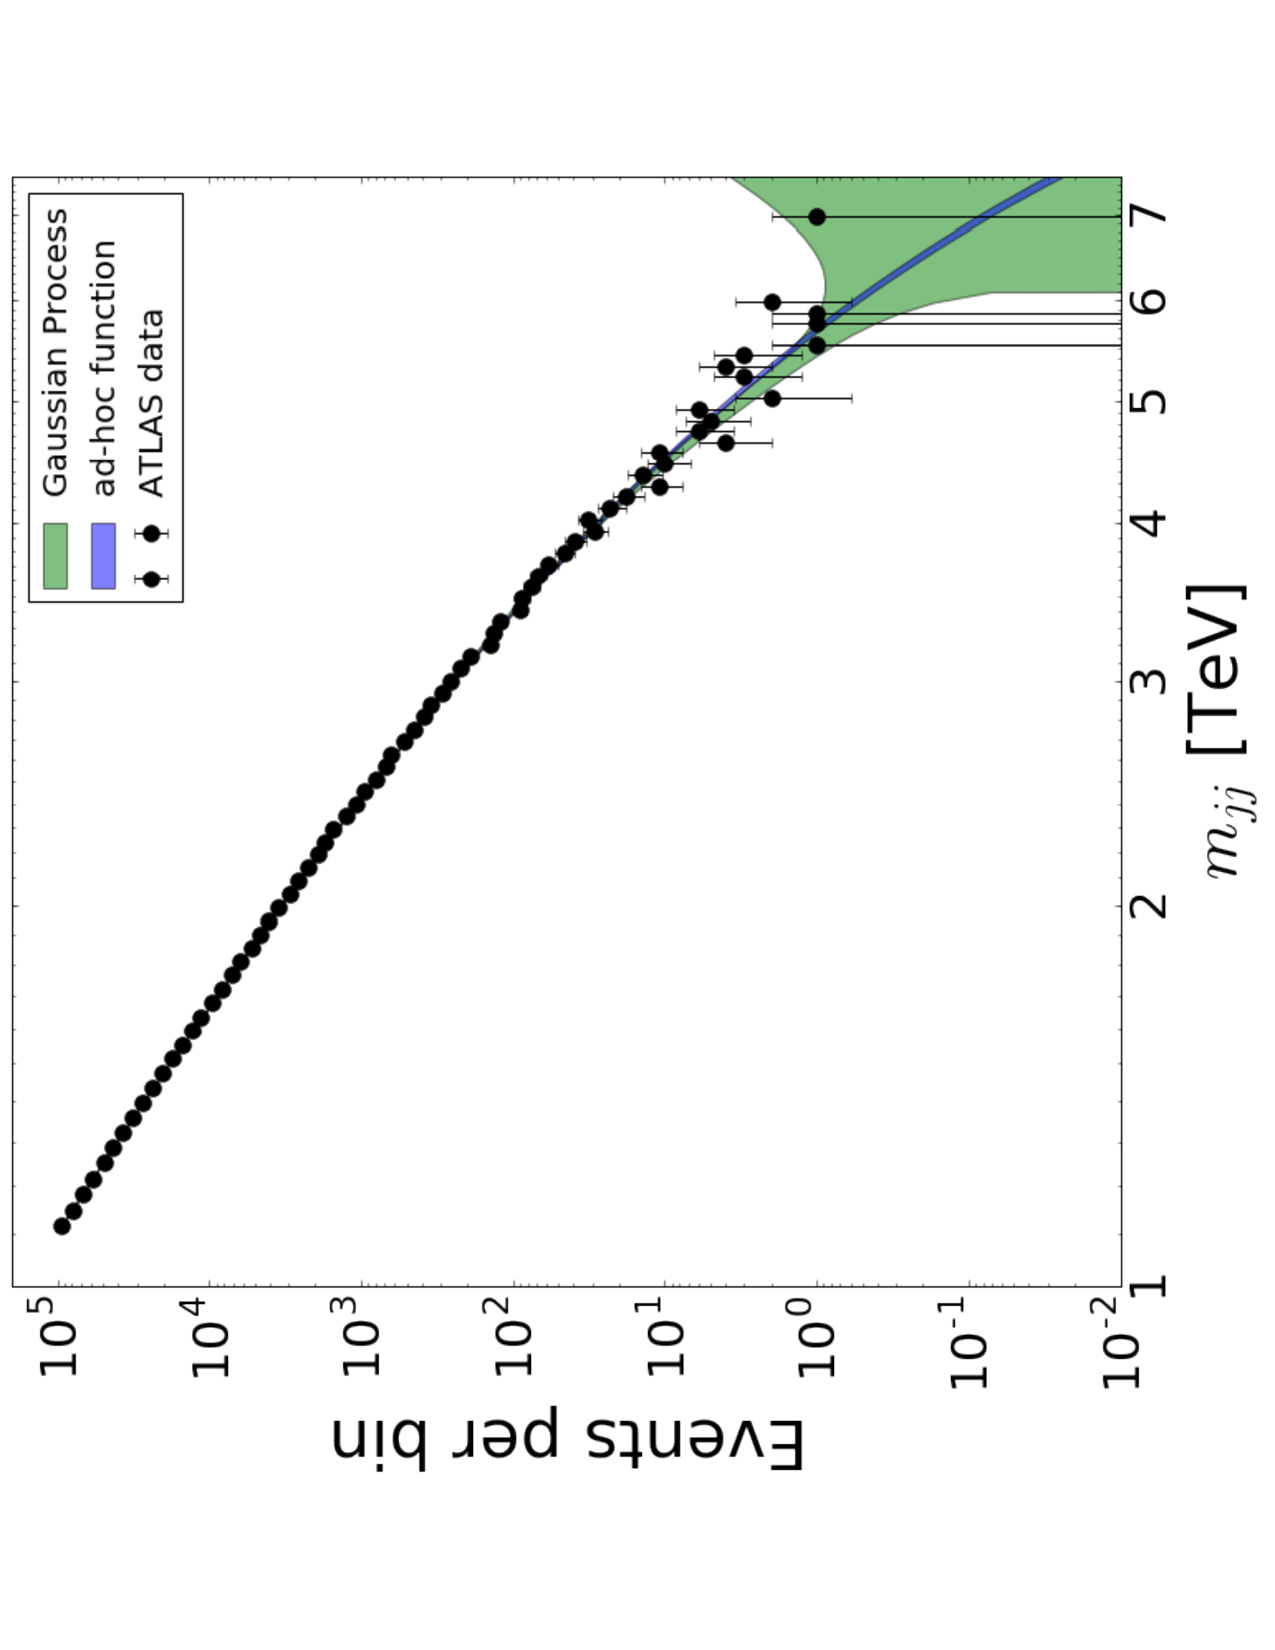
\includegraphics[width=0.58\linewidth,angle=-90]{external_figs/frate2017/FFGPonToys.pdf}
  \caption{Toy-spectrum mean and $\pm1\sigma$ background bands.}
\end{subfigure}

\vspace{0.8em}

\begin{subfigure}[t]{0.46\linewidth}
\centering
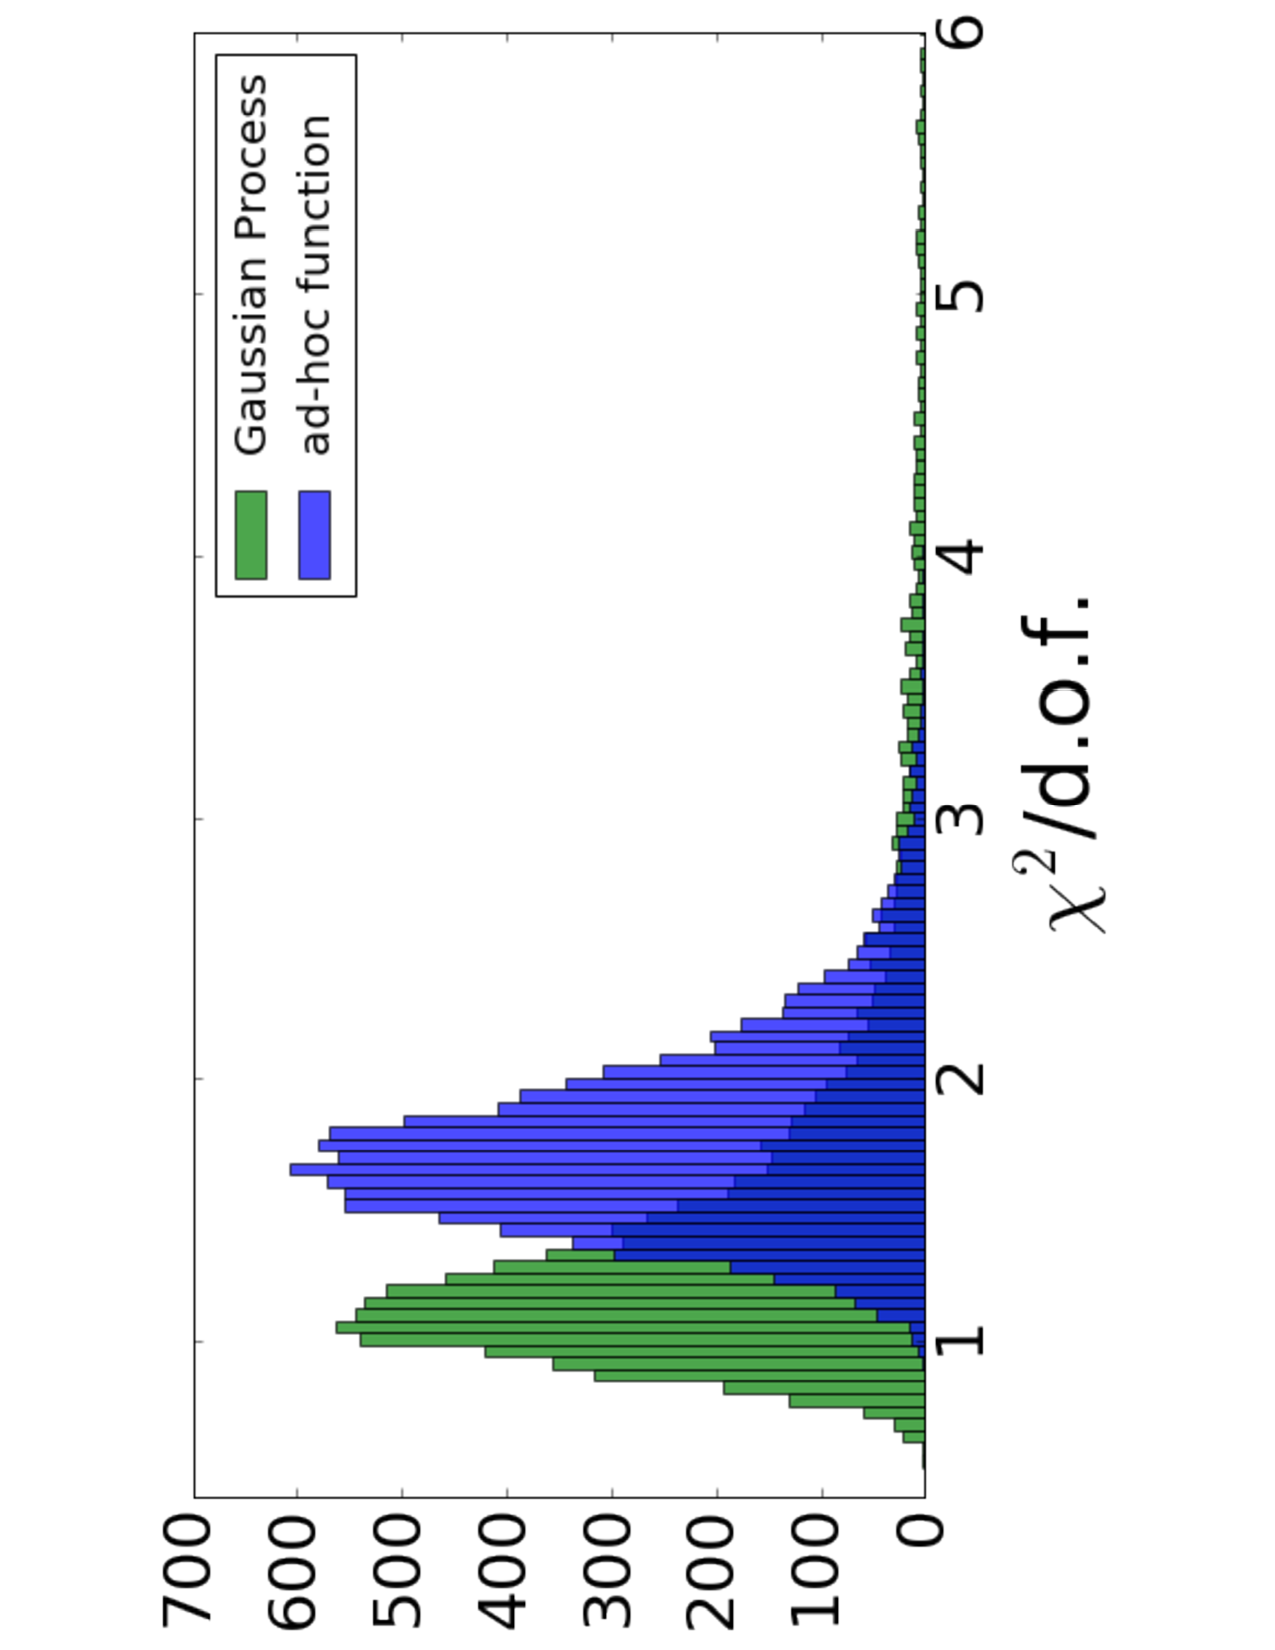
\includegraphics[width=0.76\linewidth,angle=-90]{external_figs/frate2017/chi2.pdf}
\caption{Toy goodness-of-fit distributions.}
\end{subfigure}
\hfill
\begin{subfigure}[t]{0.46\linewidth}
\centering
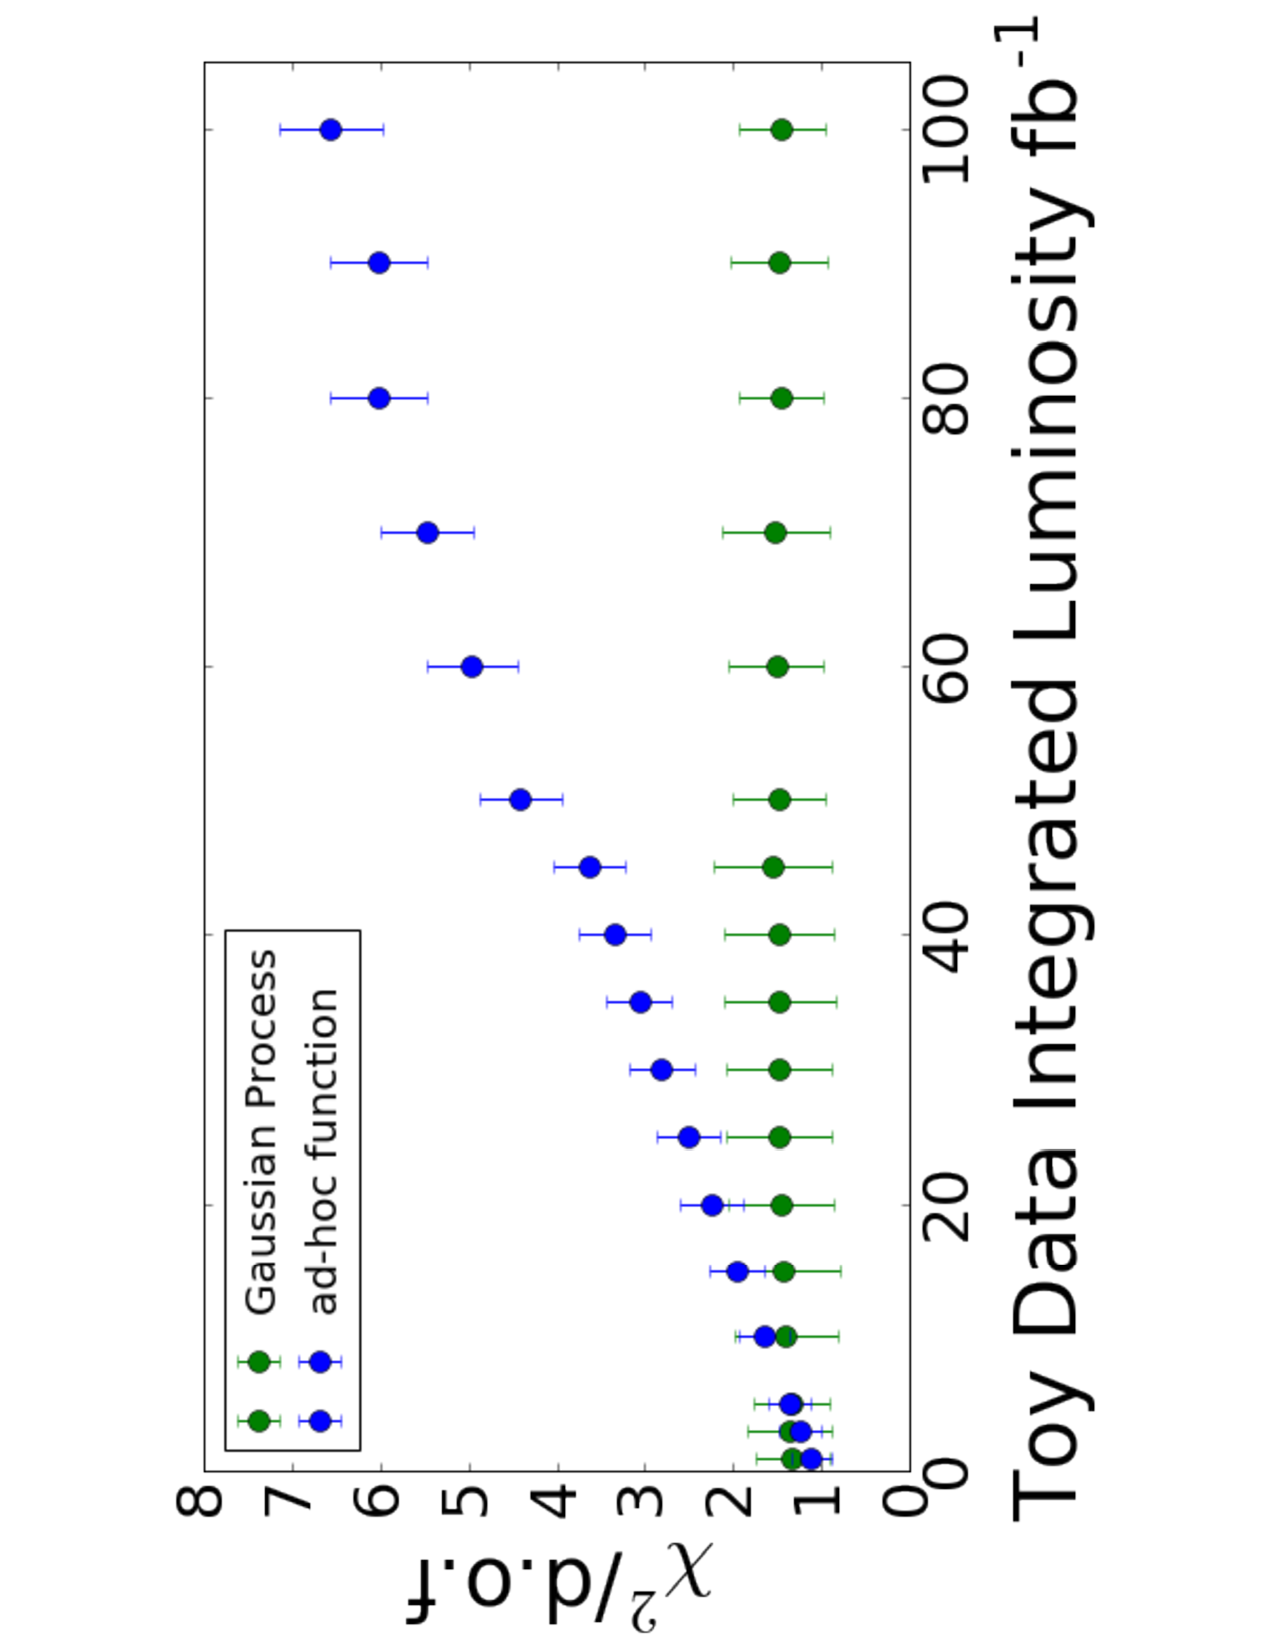
\includegraphics[width=0.76\linewidth,angle=-90]{external_figs/frate2017/lumivschi2.pdf}
\caption{Goodness of fit versus effective luminosity.}
\end{subfigure}
\caption{Methodological comparison between Gaussian-process and ad-hoc functional-form
background modeling reproduced from Ref.~\cite{FrateGP2017}. The panels show that, in
the 2017 dijet toy study, the GP retained an accurate smooth-background description
while the fixed functional form became increasingly strained as the effective
statistical precision improved.}
\label{fig:frate-gp-vs-adhoc}
\end{figure}

The later CMS-oriented GPR signal-extraction study by Gandrakota \textit{et al.}
provides the closest methodological bridge to the present implementation: choose a
kernel class, condition the GP on binned count data, compare candidate kernels against
the smooth background structure, and then separate a localized signal component from
the inferred background in a reproducible statistical workflow \cite{Gandrakota2023}.
The HPS analysis adopts that framework in a form matched to a fixed-target
prompt-resonance search. It trains the GP in log-mass/log-count space, removes the
test-mass window from training, ties the allowed length scale to the detector
resolution, converts the posterior prediction back into count space, and carries the
resulting mean vector and covariance matrix into the local profile likelihood. As
detailed in Section~\ref{sec:methodology}, GPR turns smooth-background interpolation
into an explicit probabilistic model that can be validated, profiled, and combined
across datasets.

Earlier HPS prompt searches used mass-window-specific background models,
window-by-window optimization, and a resonance extraction whose numerical behavior
depended on the local fit boundaries. Here, every mass hypothesis is assigned its own
GP fit on a fixed, dataset-specific support, with a narrow region around that hypothesis
excluded from training. The fit supplies a mean vector and covariance matrix for the
blinded bins. Signal extraction, local significance, modified-frequentist \CLs\ limits,
radiative-fraction conversion, and the shared-$\eps^2$ combination then follow within
one statistical framework.

This change is especially valuable for the present HPS program because one statistical
workflow must describe three campaigns with different mass ranges and detector
configurations. In v4 the tested signal hypotheses span \SIrange{19}{90}{MeV} for
2015, \SIrange{39}{180}{MeV} for 2016, and \SIrange{50}{250}{MeV} for 2021, while
the GP fit supports extend beyond those tested intervals to
\SIrange{14}{135}{MeV}, \SIrange{30}{210}{MeV}, and
\SIrange{40}{300}{MeV}, respectively. A stable GP model therefore matters both for
numerical smoothness and for carrying the same radiative-fraction and uncertainty
treatment across datasets without sacrificing narrow-resolution sensitivity. It also
motivates the combined analysis:
the minimal visible $A^\prime$ model predicts one common coupling $\eps^2$ at a given
mass, while each HPS run maps that coupling into a different expected signal yield
through its own integrated luminosity, acceptance, resolution, and radiative
normalization. The
statistical combination therefore treats $\eps^2$ as the shared parameter of interest
and multiplies the independent dataset likelihoods, profiling the dataset-specific
background nuisance parameters separately. In this common-parameter construction,
datasets with better local signal-to-background leverage carry more information, while
weaker channels still contribute correctly; the gain in sensitivity comes from adding
independent likelihood information for the same minimal-model signal rather than from
averaging separate limits after the fact.

\subsection{Scope of this note}

This note documents the HPS prompt $A^\prime \rightarrow e^+e^-$ GPR analysis. It
emphasizes three related physics inputs: the detector apparatus that defines the mass
resolution and acceptance, the dataset-specific radiative-fraction normalization that
converts signal yield into
$\eps^2$, and the profile-likelihood methodology used to quote local significance and
upper limits. The 2015 data are fully unblinded and are used as the most mature
validation sample. The v4 result combines the full 2015 and 2016 samples with the
reviewed 2021 10\% sample in one shared-coupling likelihood. The 2021 contribution
remains a staged partial-data result rather than the final full-2021 unblinding.

The 2019 physics run is mentioned only as part of the detector evolution from the
2015/2016 baseline configuration to the 2019/2021 upgraded configuration. Its data do
not enter the v4 prompt-resonance analysis.

Two result states are kept distinct. The accepted v4.2 three-campaign analysis uses a
40--300~MeV GP support for the 2021 sample and is unchanged. The later v4.9.5 pass is a
separate 2021-only analysis of the native 10\% sample: it retains the 50--250~MeV search
interval and freezes a 36--300~MeV GP support after the support-edge continuation. That
choice follows the practical rule adopted after the first phase of the conditional toy
study. It is neither a direct coverage qualification nor a replacement for the v4.2
combined-analysis card, and it does not alter the interpretation of the observed
65~MeV feature in that result.
